%%%%%%%%%%%%%%%%%%%%%%%%%%%%%%%%%%%%%%%%%
% Short Sectioned Assignment
% LaTeX Template
% Version 1.0 (5/5/12)
%
% This template has been downloaded from:
% http://www.LaTeXTemplates.com
%
% Original author:
% Frits Wenneker (http://www.howtotex.com)
%
% License:
% CC BY-NC-SA 3.0 (http://creativecommons.org/licenses/by-nc-sa/3.0/)
%
%%%%%%%%%%%%%%%%%%%%%%%%%%%%%%%%%%%%%%%%%

%----------------------------------------------------------------------------------------
%	PACKAGES AND OTHER DOCUMENT CONFIGURATIONS
%----------------------------------------------------------------------------------------

\documentclass[paper=letter, fontsize=11pt]{scrartcl} % A4 paper and 11pt font size

\usepackage[T1]{fontenc} % Use 8-bit encoding that has 256 glyphs
\usepackage{fourier} % Use the Adobe Utopia font for the document - comment this line to return to the LaTeX default
\usepackage[english]{babel} % English language/hyphenation
\usepackage{amsmath,amsfonts,amsthm} % Math packages

\usepackage[cm]{fullpage}
\usepackage{color}
\usepackage{graphicx}
\usepackage{caption}


\usepackage{sectsty} % Allows customizing section commands
\allsectionsfont{\centering \normalfont\scshape} % Make all sections centered, the default font and small caps




%\numberwithin{equation}{section} % Number equations within sections (i.e. 1.1, 1.2, 2.1, 2.2 instead of 1, 2, 3, 4)
%\numberwithin{figure}{section} % Number figures within sections (i.e. 1.1, 1.2, 2.1, 2.2 instead of 1, 2, 3, 4)
%\numberwithin{table}{section} % Number tables within sections (i.e. 1.1, 1.2, 2.1, 2.2 instead of 1, 2, 3, 4)



%----------------------------------------------------------------------------------------
%	TITLE SECTION
%----------------------------------------------------------------------------------------

\newcommand{\horrule}[1]{\rule{\linewidth}{#1}} % Create horizontal rule command with 1 argument of height

\title{	
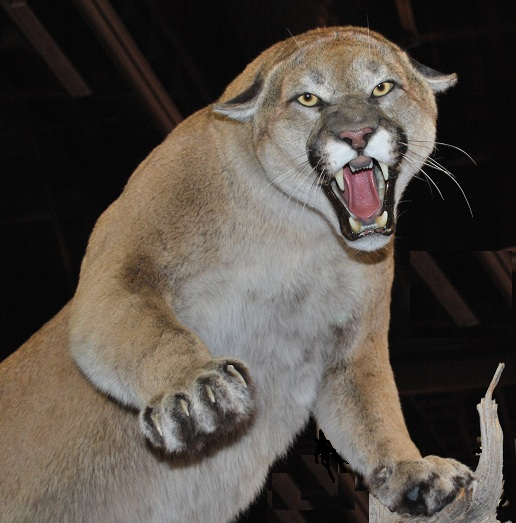
\includegraphics[width=3cm]{Cougar_Nevada}
\normalfont \normalsize 
%\textsc{APC 524} \\ [25pt] % Your university, school and/or department name(s)
\horrule{0.5pt} \\[0.4cm] % Thin top horizontal rule
\LARGE COUGAR (\textbf{CO}de \textbf{U}sually \textbf{G}enerates \textbf{A}xisymmetric \textbf{R}econstruction), \\ \Large An MHD Equilibrium Reconstruction Code:  Design Document\\ % The assignment title
\horrule{2pt} \\[0.5cm] % Thick bottom horizontal rule
}

\author{Peter Bolgert (pbolgert@pppl.gov), Jonathan Ng (wng@pppl.gov), \\ Elizabeth Paul (epaul@princeton.edu), Jacob Schwartz (jschwart@pppl.gov)} % Your name

\date{\normalsize\today} % Today's date or a custom date

\begin{document}

\maketitle % Print the title

%----------------------------------------------------------------------------------------
%	Section 1
%----------------------------------------------------------------------------------------

\section{Overview}

\subsection{MHD equilibrium}

In magnetohydrodynamic (MHD) theory, a plasma equilibrium is described by the equation $\mathbf{\nabla} p = \mathbf{J} \times \mathbf{B}$, where $p$ is the scalar plasma pressure, $\mathbf{J}$ is the current density, $\mathbf{B} = \mathbf{\nabla} \times \mathbf{A}$ is the magnetic field, and $\mathbf{A}$ is the vector potential for the magnetic field.  We work in cylindrical coordinates $(R, \phi, Z)$, and the plasma is assumed to be axisymmetric, i.e., $\partial / \partial \phi = 0$.

By introducing new functions $\Psi(R,Z) \equiv -R A_{\phi}$ (called the flux function) and $g(R,Z) \equiv R \big(\frac{\partial A_R}{\partial Z} - \frac{\partial A_Z}{\partial R}\big)$, we can rewrite the equilibrium equation in the following form, known as the Grad-Shafranov equation:
\begin{equation}
\Delta^{*} \Psi + \mu_0 R^2 \frac{dp}{d\Psi} + g \frac{dg}{d\Psi} = 0,
\end{equation}
where $\Delta^{*} \equiv R^2 \mathbf{\nabla} \cdot \frac{1}{R^2} \mathbf{\nabla}$ is called the toroidal elliptic operator. $p(\Psi)$ and $g(\Psi)$ are functions of $\Psi(R,Z)$, the quantity that we are trying to solve for.  Thus $p(\Psi)$ and $g(\Psi)$ must be given (along with boundary conditions) for the problem to be fully specified.  Once the equation is solved, any other quantity of interest ($\mathbf{J}$, $\mathbf{B}$, etc.) can be calculated.  

\begin{figure}
\centering
\captionsetup{justification=centering,margin=3cm}
\caption[caption]{Cylindrical coordinates $(R,\phi,Z)$.  Taken from "Computational Methods in Plasma Physics," Stephen Jardin.}

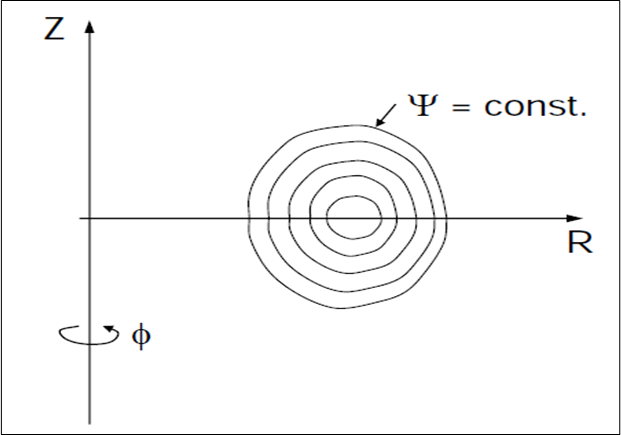
\includegraphics[width=0.35\textwidth]{coordinates}

\end{figure}

Without going into too much detail, it should be stated that the best MHD equilibria for confining plasmas are those which contain nested surfaces of constant $\Psi$ (known as flux surfaces), as in Figure 1.  It can be shown that a magnetic field line will always point tangentially to a given flux surface.  Since charged particles in the plasma follow field lines, the particles will stay on constant flux surfaces, resulting in good confinement.    



\subsection{Equilibrium Reconstruction}

In a tokamak experiment, one of the researchers' primary goals is to calculate the flux function $\Psi(R,Z)$ at various times throughout the discharge.  However, in this case, the functional forms of $g(\Psi)$ and $p(\Psi)$ are unknown.  Instead we must rely on a finite number of experimental measurements of $\Psi$ taken near the plasma boundary.  The approximate calculation of the flux function from these experimental measurements is known as Equilibrium Reconstruction.  

Equilibrium reconstruction is crucial for interpreting the results of experiments. In addition, the reconstructed equilibria are often used as inputs to other codes, such as stability codes or transport codes.  

Our program will be able to solve the Grad-Shafranov equation 1) when $p(\Psi)$ and $g(\Psi)$ are specified, and 2) when only experimental measurements are available.

\subsection{Algorithm when $p(\Psi)$ and $g(\Psi)$ are specified}



First rewrite the Grad-Shafranov equation as
\begin{equation}
\Delta^{*}\Psi = \mu_0 R J_{\phi} (R, \Psi),
\end{equation}
where $\mu_0 R J_{\phi} (R,\Psi) = - \big(\mu_0 R^2 \frac{d p}{d\Psi} + g \frac{d g}{d\Psi}\big)$.

Since the problem is non-linear (the right-hand-side of Eq.~(2) depends on $\Psi$), we use an iterative approach.  At each level of iteration, we solve a finite difference version of 
\begin{equation}
\Delta^{*}\Psi^{n} = \mu_0 R J_\phi (R, \Psi^{n-1}),
\end{equation}
where $n$ denotes the iteration level. At each level, the previous iteration's result for $\Psi$ is plugged into the right-hand-side of Eq.~(3).  This continues until the solution converges.  The linearized finite difference equation can be solved via transform methods or multi-grid methods.

There is an additional nonlinearity relating to the boundary conditions.  Suppose that there are $N_c$ external coils outside of the computational boundary.  The flux function evaluated on the computational boundary $\Psi_b$ is then due to the plasma itself and the external coils:
\begin{equation}
\Psi^m_b (R',Z') = \int_{b} \frac{dl}{R} G(R,Z; R',Z') \frac{\partial U^m}{\partial n} + \sum_{i=1}^{N_c} G(R_i^c,Z_i^c; R',Z') I_i,
\end{equation}
where $G$ is the Green's Function for the elliptic operator $\Delta^{*}$ (known analytically and stored in a look up table), $(R_i^c,Z_i^c)$ is the location of the $i$th coil with current $I_i$, and $U^m(R,Z)$ is a function which satisfies
\begin{align}
\Delta^{*} U^m &= \mu_0 R J_\phi (R, \Psi^{m-1}) \quad \mbox{inside the comp.~boundary} \\
U^m &= 0 \quad \mbox{on the boundary}.
\end{align}
The calculation of the boundary values using Eq.~4 is known as Von Hagenow's method (Lackner, Comp.~Phys. Comm.~12 (1976) 33-44).
The index $m$ in Eq.~(4) shows that the determination of the boundary condition is also an iterative process.  The $(m-1)$th value of $J_\phi$ is used to calculate $\Psi_b^m$.  

Given a set of boundary conditions, we can solve Eq.~(3) iteratively for $\Psi$.  This $\Psi$ is then used to calculate a new set of boundary conditions using Eq.~(4), and the process begins anew.  Ultimately, the process is a double-nested iteration which runs until the outer loop converges.  The process is depicted in Figure 2.

\begin{figure}
\centering
\captionsetup{justification=centering,margin=3cm}
\caption[caption]{Double-nested iteration loop. Taken from "Computational Methods in Plasma Physics," Stephen Jardin.}
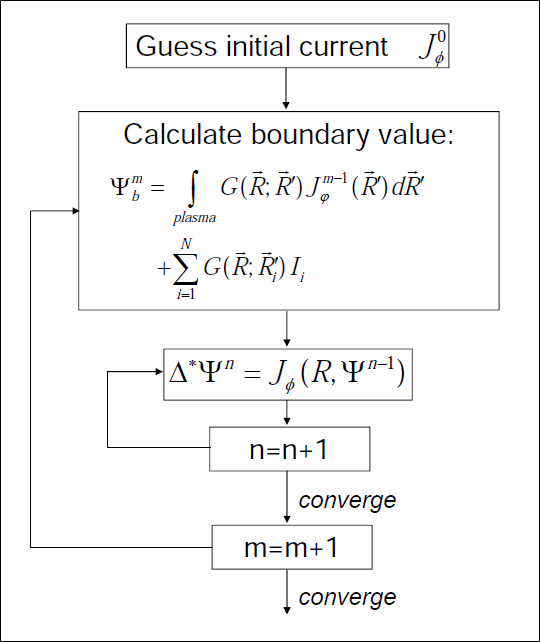
\includegraphics[width=0.45\textwidth]{algorithm}
\end{figure}

In summary, the \textbf{inputs} to the algorithm are an initial guess $J_\phi^0$ for the source function, the location of external coils $(R_i^c,Z_i^c)$ and their currents $I_i$, and the functional forms of $p(\Psi)$ and $g(\Psi)$.  The \textbf{output} is the value of $\Psi$ at each grid point in the $R-Z$ plane.  

\subsection{Algorithm using Experimental Measurements}

In an experiment, $p(\Psi)$ and $g(\Psi)$ are unknown, but suppose we have $N_l$ measurements of the flux function $\Psi_l^{meas}$ near the plasma boundary (but within the computational boundary).  

First we expand our unknown functions in terms of basis functions (which our group must still determine):
\begin{equation}
p'(\Psi) = \sum_j \alpha_j y_j(\Psi), \quad gg'(\Psi) = \sum_j \beta_j y_j(\Psi).
\end{equation}
We can then write a formula for the computed value of $\Psi$ at the location $(R_l, Z_l)$ of each experimental measurement: 
\begin{equation}
\Psi_l^{comp}(R_l, Z_l) = \int_{plasma} G(R,Z; R_l,Z_l) J_\phi(R,\Psi,\alpha_j,\beta_j) dR dZ + \sum_{i=1}^{N_c} G(R_i^c,Z_i^c; R_l,Z_l) I_i.
\end{equation}
The computed values are compared to the measured values, and the minimization of an error function determines the values of $\alpha_j, \beta_j$ at that stage in the algorithm.   

Thus, the algorithm described in Section 1.4 is identical to that described in Section 1.3 (and depicted in Fig.~2), except that each time $\Psi$ is updated in the inner ($n$) loop, we also update the values of $\alpha_j, \beta_j$.  In summary, the \textbf{inputs} to the algorithm are an initial guess $J_\phi^0$ for the source function, the location of external coils $(R_i^c,Z_i^c)$ and their currents $I_i$, and the location of the experimental measurements $(R_l,Z_l)$ and their values $\Psi_l^{meas}$.  The \textbf{output} is the value of $\Psi$ at each grid point in the $R-Z$ plane.  



%----------------------------------------------------------------------------------------
%	Section 2
%----------------------------------------------------------------------------------------

\section{Code Organization}

The program will be written in C++ with the visualization carried out separately using Python. The solver would be called from the command line, with options to set the parameters of the simulation. Input data, such as the locations of external coils, will be contained in text files. 
\\

Output will be written to hdf5 files, which will require installation of the hdf5 library.  By default, the output consists of the grid and flux function.  Other quantities, such as the toroidal current density, can be selected in the input file.\\

The following C++ interfaces will be required and should be self-contained
\begin{itemize}
\item Elliptic solver - This is used to invert the elliptic operator $\Delta^*$ and solve for $\Psi$, given the source functional in the Grad-Shafranov equation [Eq.~(2)]. This should allow the swapping in of external matrix solvers and the implementation of a multi-grid method if time permits. There should be potential for parallelization here. If there is matching to experimental data, the least-squared calculation of the parameters $\alpha_j$ and $\beta_j$ from Eq.~(8) will be performed here. 
\item Boundary condition solver - Used to determine $\Psi$ on the computational boundary given external currents [Equation (4)]. Again this should allow different algorithms to be implemented. There should be potential for parallelization here. 
\item Grad-Shafranov solver - Given input currents and equations, this will perform the call to the elliptic and boundary solvers and perform the iterations until it converges.
\item Input parsing - To read the source currents and parameters from an input file.
\item Output - To write the output to an hdf5 file. Support for other formats could be added eventually.
\end{itemize}

For the visualization in Python, the numpy and matplotlib libraries will be used. Functions to extract the data, subsets of the data and calculation of common plasma parameters will be provided. Only basic visualization such as plotting contours and 1-D cuts will be built in, since users will likely wish to evaluate the data using their own methods based on what they are studying. \\

The current research reconstruction code EFIT solves for approximately 250 equilibria in 20 seconds for the DIII-D tokamak. This should be a performance goal to aim for. \\

External libraries
\begin{itemize}
\item HDF5 will be required for I/O. This can be downloaded for free. The Python version h5py will be used for visualization.
\item Eigen or one of the many free BLAS variants can be used for matrix operations.
\item MPI will be used for any parallelization we add to the code. 
\item Matplotlib and numpy will be used for visualization.
\end{itemize}

%----------------------------------------------------------------------------------------
%	Section 3
%----------------------------------------------------------------------------------------

\section{User Interface}

The program will be called from the command line and take as an argument an input (text) file. 

The text file will contain key-value pairs including
\begin{itemize}
\item Switch controlling initial conditions of solver - either $\Psi_B$, $p(\Psi)$ and $g(\Psi)$, or external coil data are specified. 
\item Path to a file describing external currents (from coils outside the plasma) and experimental measurements of $\Psi$ at various points outside the plasma.
\item Path to a file with the $p(\Psi)$ and $g(\Psi)$ functions, when they are specified.
\item Path to a file with a specified boundary $\Psi$: this will be useful in testing the inner loop.
\item Initial guess for $J_\phi$. 
\item Maximum iterations and convergence requirements for inner and outer loops. 
\item Whether to output for every $n$ or $m$ (these will be useful in debugging / so a user can watch the solution converge)
\item Whether to output $\mathbf{B}$, $\mathbf{J}$, $p$ and $q$ as well as $\Psi$ for each cell in the final output.
\end{itemize}

For some of these key-value pairs, there may be default values if none is specified, while for others, the program will terminate with an error message if no key/value is specified.

The input file of external currents will be a tab-separated table of radial location R (meters), vertical coordinate Z (meters) and I (amps) for each poloidal field coil.

The input file of experimental magnetic field measurements will be similar: a tab-separated table of R, Z, and measured $\Psi$.

Our output will be in the hdf5 format. The file will include the calculated solution for $\Psi$ and also (if the user specifies) tables for $\mathbf{B}$, $\mathbf{J}$, $p$, and/or $q$. If the user so specifies, each inner and /or outer loop's result for $\Psi$ will also be output to this file.

In order to read the hdf5 files, a Python visualizer using matplotlib will be written. It will show contour plots for the tables in the output file and also be able to take slices through the tables at the machine midplane.

%----------------------------------------------------------------------------------------
%	Section 4
%----------------------------------------------------------------------------------------

\section{Schedule and Division of Labor}

\subsection{Schedule}

\textbf{November 28, 2014 - Detailed Project Map}
\begin{itemize}
\item Illustrate the code organization through a visual map showing the connection between each of our major classes. 
\item Set up documentation browser of project with Doxygen.
\item Clearly define algorithms used: basis functions for reconstruction, finite difference solver, boundary condition solver.
\item Finalize libraries needed.
\end{itemize}

\textbf{December 5, 2014 - Prototype}
\begin{itemize}
\item Implement user interface. 
\item Implement input with text file. User defines output type along with algorithms used, number of iterations, etc.  The initial current approximation, $J^0_{\phi}$, is specified along with $p(\Psi)$ and $g(\Psi)$ or experimental measurements of $\Psi$. 
\item Implement output to a file and/or matplotlib: output is dumped to files and user can implement our plotting modules to generate plots of $\Psi$ as well as related quantities and convergence data. 
\item Implement main loop with empty function calls. Outline which functions need to be written and what libraries are used. 
\end{itemize}

\textbf{December 19, 2014 - Alpha Version}
\begin{itemize}
\item Implementation of main loop with testing: comparison with analytic solution, convergence testing, and performance testing. 
\item Implementation of finite difference method elliptic solver.
\item Implementation of boundary flux ($\Psi_b$) solver using Von Hagenow's method. 
\end{itemize}

\textbf{January 15, 2015 - Final Version}
\begin{itemize}
\item Reconstruction of $p(\Psi)$ and $g(\Psi)$ from magnetic data. 
\item Implement multi-grid method or other alternate elliptic solver. 
\item Parallelization with MPI.
\end{itemize}

\subsection{Division of Labor}
\begin{itemize}
\item Peter: Boundary condition solver, calculation of $(\alpha_j,\beta_j)$ from experimental data.
\item Jonathan: Output, Python visualization program.
\item Elizabeth: Elliptic solver
\item Jacob: Input, Testing, Grad-Shafranov solver
\end{itemize}

%----------------------------------------------------------------------------------------
%	Section 5
%----------------------------------------------------------------------------------------

\section{Risks}

Although the scope of the project we have outlined is rather large, it should be modularized such that each portion of the project can be fully implemented and tested independently - elliptic solver, boundary solver, possible multi-grid, etc. One of our greatest risks may be realizing that we were overly ambitious. In this case, we may decide that implementation of the multi-grid method is not feasible within our time frame. While our performance may be reduced in this case, we would still have produced a fairly substantial MHD equilibrium solver. We could additionally decide that it may be more realistic to implement another elliptic solver, such as an alternative finite difference method, rather than a multi-grid. Additionally, depending on our performance concerns, it may be important to implement parallelization earlier than described in the schedule. 

\end{document}
